\subsection{Alur Transaksi}
\label{subsection:system-flow}

Mengikuti batasan pada bagian \ref{sec:batasan-masalah}, transaksi yang akan diimplementasikan dalam sistem ini adalah transaksi \textit{write} dan \textit{read}. Sistem akan mendukung dua skema penyimpanan, yaitu replikasi dan \textit{erasure coding}, yang akan mempengaruhi alur transaksi.

\begin{figure}[!ht]
    \centering
    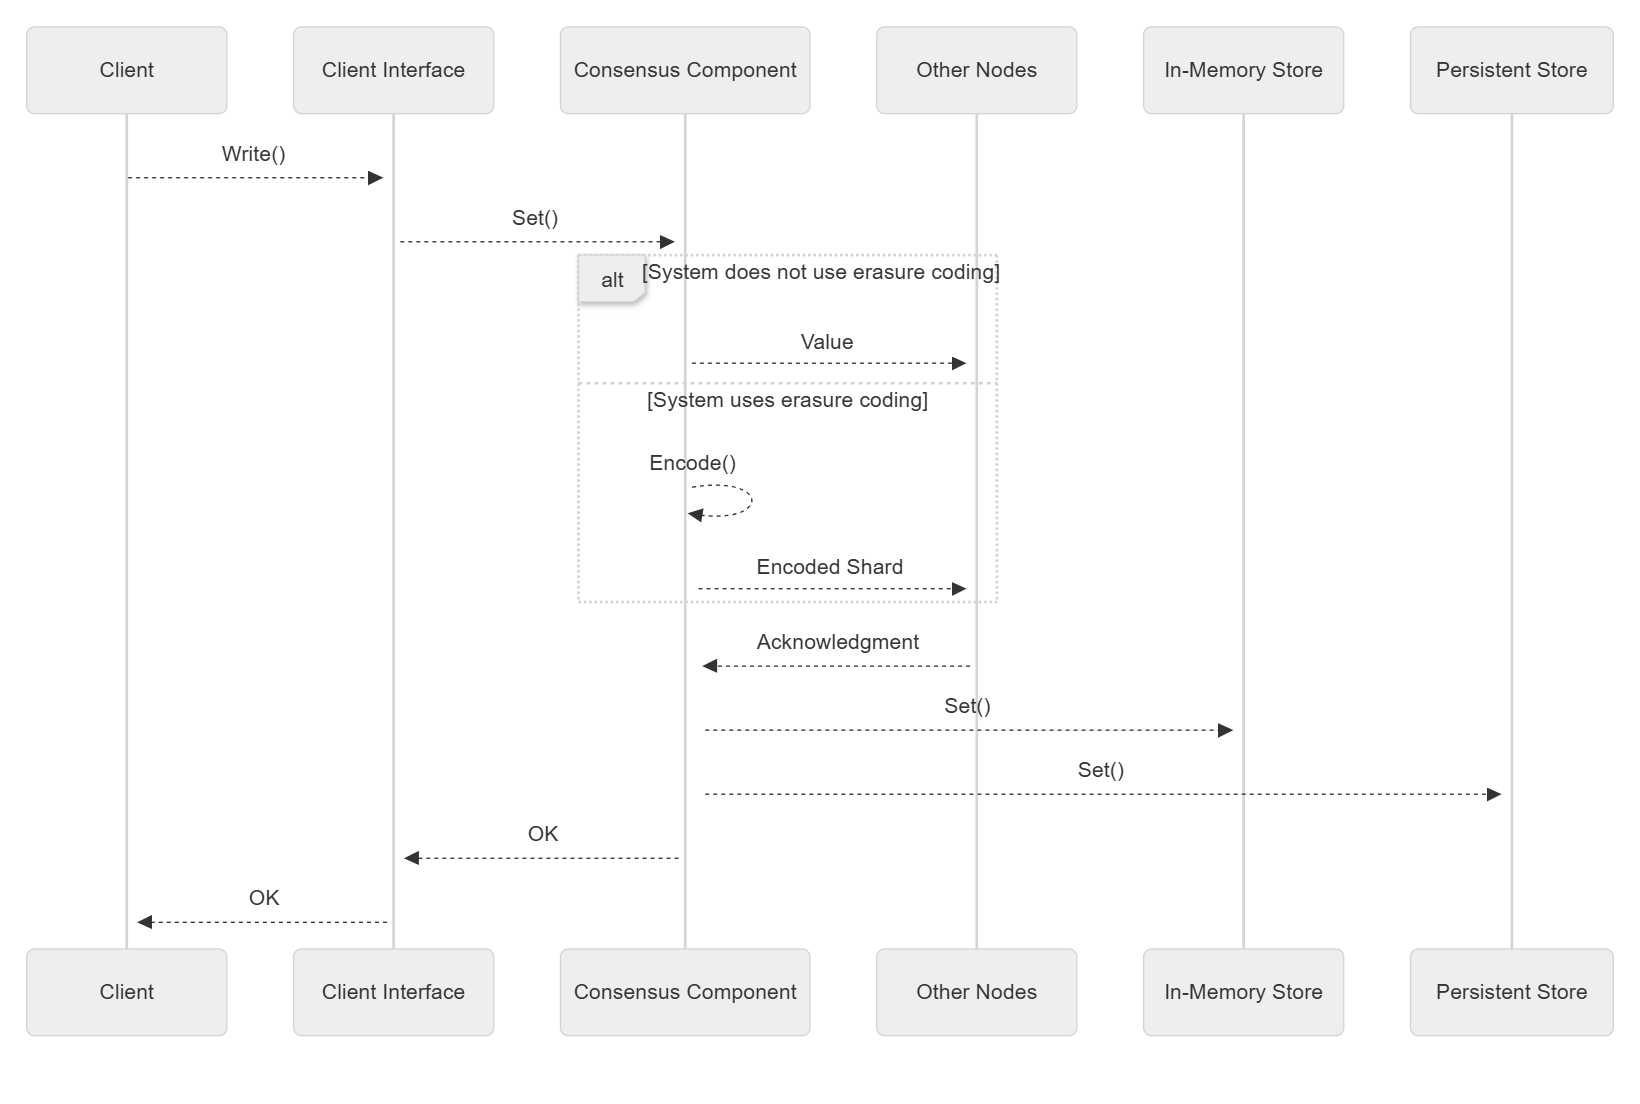
\includegraphics[width=0.95\textwidth]{resources/chapter-3/flow-write.png}
    \caption{Flow operasi \textit{write} dalam rancangan implementasi}
    \label{fig:flow-write-mermaidjs}
\end{figure}

Alur untuk transaksi \textit{write} dapat dilihat pada gambar \ref{fig:flow-write-mermaidjs} dengan \textit{request} masuk ke \textit{Node}. Node kemudian akan melakukan operasi \textit{erasure coding} lalu menyebarkan \textit{shard} ke \textit{Node} lain sesuai dengan algoritma konsensus yang digunakan. Operasi \textit{write} dianggap selesai setelah konsensus mencapai kuorum.

\begin{figure}[!ht]
    \centering
    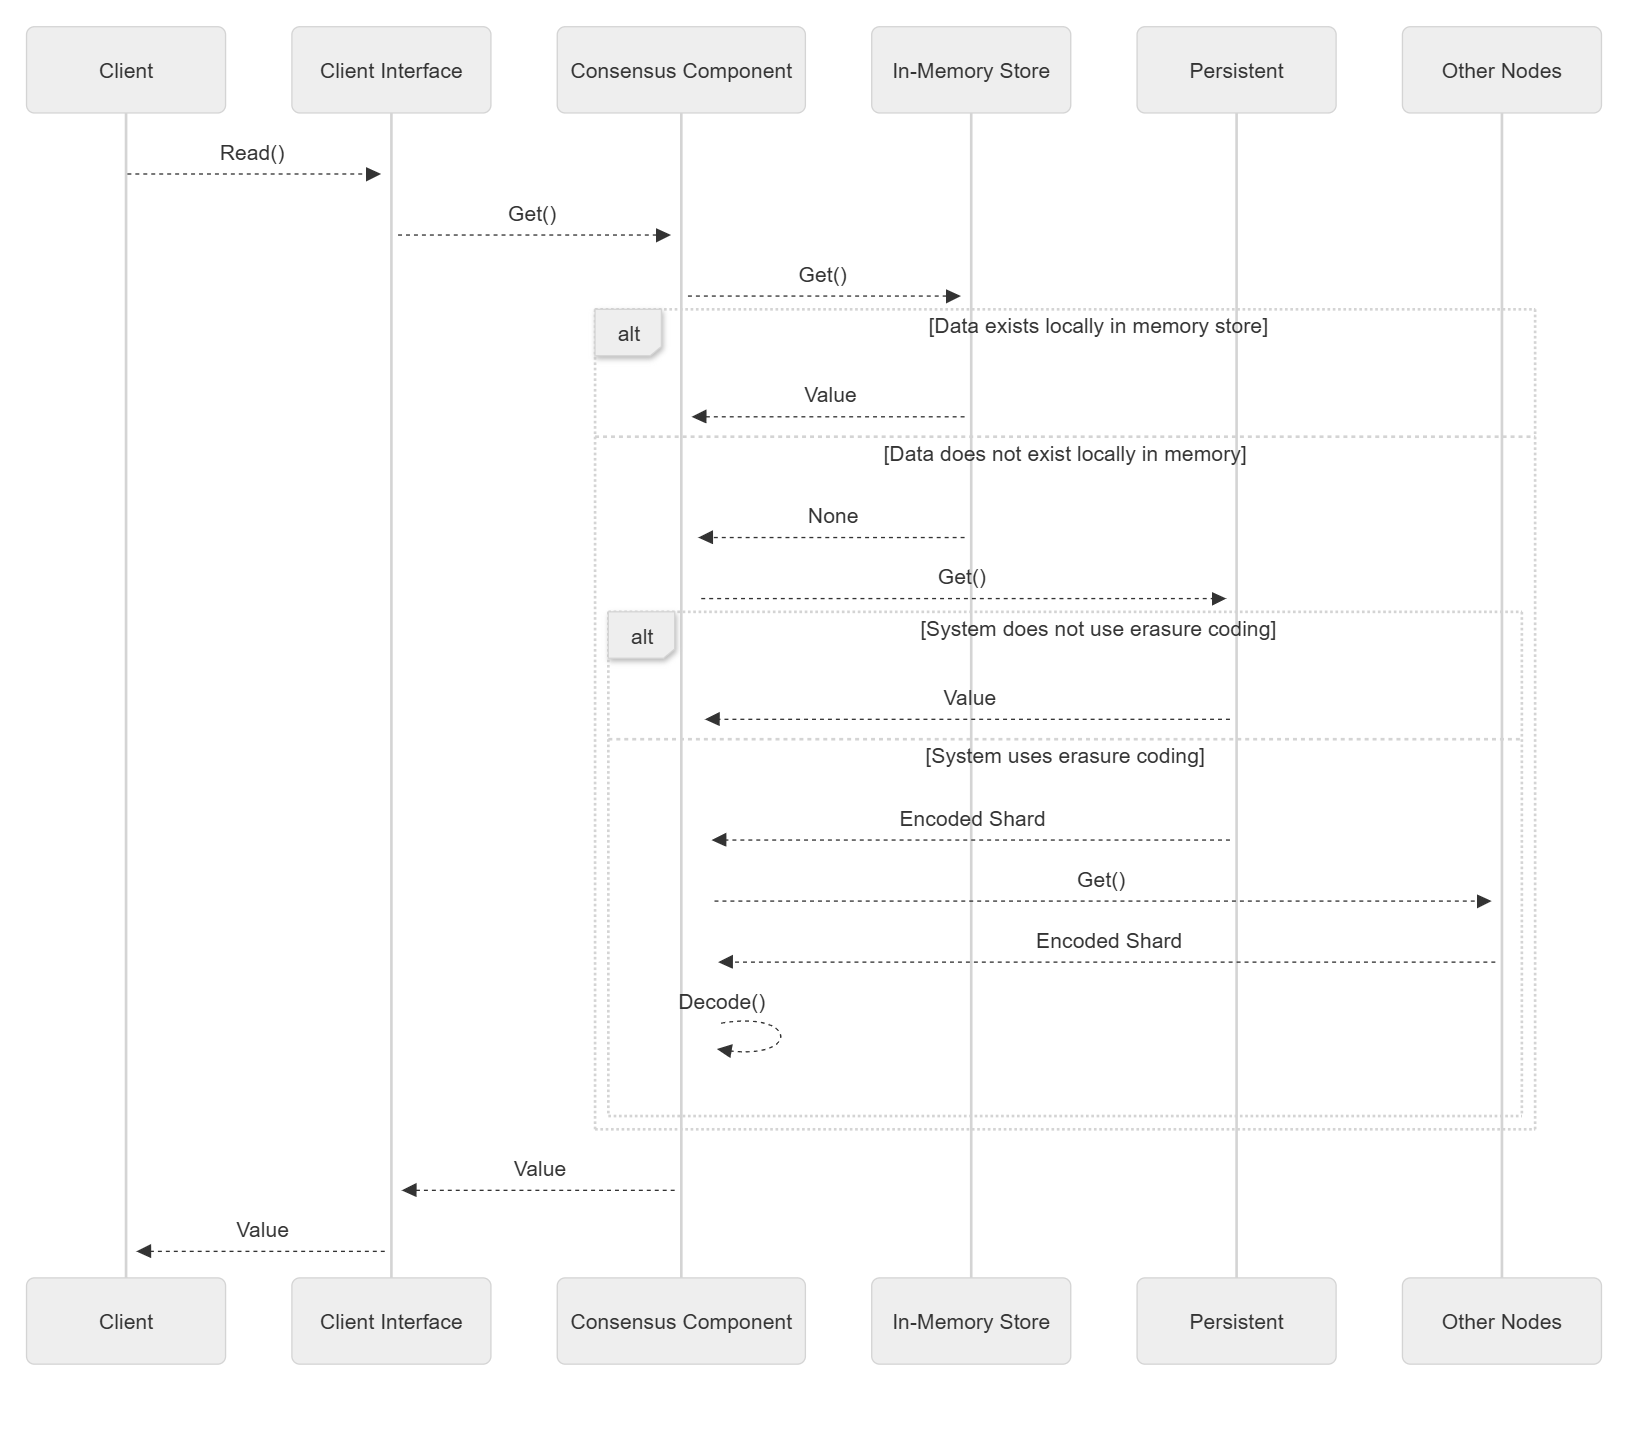
\includegraphics[width=0.95\textwidth]{resources/chapter-3/flow-read.png}
    \caption{Flow operasi \textit{read} dalam rancangan implementasi}
    \label{fig:flow-read-mermaidjs}
\end{figure}

Alur untuk transaksi \textit{read} dapat dilihat pada gambar \ref{fig:flow-read-mermaidjs} dengan \textit{request} masuk ke \textit{Node} yang tersedia. \textit{node} melakukan operasi \textit{read} pada \textit{key-value store} dan mengembalikan hasil operasi ke \textit{client} jika tersedia. Jika tidak, maka \textit{Node} melakukan rekonstruksi data dari \textit{erasure-coded persistent data} yang tersebar pada \textit{node-node} lainnya. Pada replikasi, data diambil dari \textit{Node} lain yang memiliki data yang sama.